%%%%%%%%%%%%%%%%%%%%%%%%%%%%%%%%%%%%%%%%%%%%%%%%%%%%%%%%%%%%%%%%%%%%%%
%
% Institut für Rechnergestuetzte Automation
% Forschungsgruppe Industrial Software
% Arbeitsgruppe ESSE
% http://security.inso.tuwien.ac.at/
% lva.security@inso.tuwien.ac.at
%
% Version 2012-10-17
% 
%%%%%%%%%%%%%%%%%%%%%%%%%%%%%%%%%%%%%%%%%%%%%%%%%%%%%%%%%%%%%%%%%%%%%%

\documentclass[12pt,a4paper,titlepage,oneside]{scrartcl}
\usepackage{esseProtocol}

%%%%%%%%%%%%%%%%%%%%%%%%%%%%%%%%%%%%%%%%%%%%%%%%%%%%%%%%%%%%%%%%%%%%%%
%
% FOR STUDENTS
%
%%%%%%%%%%%%%%%%%%%%%%%%%%%%%%%%%%%%%%%%%%%%%%%%%%%%%%%%%%%%%%%%%%%%%%

% Group number or "0" for Lab0
\newcommand{\gruppe}{5}
% Date
\newcommand{\datum}{05.06.2013}
% valid values: "Lab0", "Lab1" (be sure to use Uppercase for first character)
\newcommand{\lab}{Lab1}

% name of course, for example: "IT Security in Large IT Infrastructures", "Security for Systems Engineering", "Introduction to Security"
\newcommand{\lvaname}{IT Security in Large IT Infrastructures}
% number of course, for example: "183.633", "183.637", "183.594"
\newcommand{\lvanr}{183.633}
% year and term, for example: "SS 2012", "WS 2012", "SS 2013", etc.
\newcommand{\semester}{SS 2013}

% Student data in Lab0 or 1. student of group in Lab1
\newcommand{\studentAName}{Michael Heil}
\renewcommand{\studentAMatrnr}{0826358}
\newcommand{\studentAEmail}{e0826358@student.tuwien.ac.at}

% 2. student of group in Lab1, for Lab0 or if your group has less students, remove this 3 lines
\newcommand{\studentBName}{Lukas Puschmann}
\renewcommand{\studentBMatrnr}{0825354}
\newcommand{\studentBEmail}{e0825354@student.tuwien.ac.at}

% 3. student of group in Lab1, for Lab0 or if your group has less students, remove this 3 lines
\newcommand{\studentCName}{Dominik Amon}
\renewcommand{\studentCMatrnr}{1228536}
\newcommand{\studentCEmail}{e1228536@student.tuwien.ac.at}


%%%%%%%%%%%%%%%%%%%%%%%%%%%%%%%%%%%%%%%%%%%%%%%%%%%%%%%%%%%%%%%%%%%%%%
%
% DO NOT CHANGE THE FOLLOWING PART
%
%%%%%%%%%%%%%%%%%%%%%%%%%%%%%%%%%%%%%%%%%%%%%%%%%%%%%%%%%%%%%%%%%%%%%%

\newcommand{\dokumenttyp}{Report \lab}

\begin{document}

\maketitle
\setcounter{section}{0}
\setcounter{tocdepth}{2}
\tableofcontents

%%%%%%%%%%%%%%%%%%%%%%%%%%%%%%%%%%%%%%%%%%%%%%%%%%%%%%%%%%%%%%%%%%%%%%
%
% CONTENT OF DOCUMENT STARTS HERE
%
%%%%%%%%%%%%%%%%%%%%%%%%%%%%%%%%%%%%%%%%%%%%%%%%%%%%%%%%%%%%%%%%%%%%%%

\section{lab1a - Safety Objectives}
Security is the core requirement to this software system. In this chapter we will list and explain the
safety objectives of the system as a whole as well as its implications to its separate components. The order
of the targets has no impact on their importance.


\subsection{Authorization}
Despite the fact that authorization represents the basic functionality of this system, this goal is also
an important non-functional issue concerning the communication of the different components themselves. Consequently, all components,
especially those outside of immediate control, but also those within system boundaries are subject to strict authorization.

A strategy to achieve this goal is to follow the \emph{complete mediation} design principle which states that each and
every request needs to be verified instead of keeping a cached authorization result. As such, the performance might suffer
a bit but regarding security this is a must.


\subsection{Authenticity}
Similar to \emph{authorization}, authenticity is important for intra- and inter-communication of all components. To
ensure authenticity the \emph{complete mediation} principle provides support to a comprehensive certificate-based authentication
system. These certificates are managed and replaced at regular intervals.

The most vulnerable spot are the external interfaces of the \emph{authorization and object management} as an intruder could get
a) information about the access rights (confidentiality) and b) change any of these data (integrity). Therefore it is important to impose
a strict authentication and autorization policy here.

Functional authentication will basically be realized using a RFID-chip each employee or person who wishes to gain access has to carry.
In normal situations the person to be authorized has to put the chip onto or in front of a reader and provide his six digit pin
(which has to be changed every six months). There will also be the possibility to lock a chip if lost similar to a credit card.
For critical secured objects an additional iris-scan will be conducted and compared to the data stored on the chip.
More information is to follow in a later chapter.

Generally no component in the system must ever trust any component from beyond the border. The possibility is always there that
it was replaced or reconfigured to act in a malicious way. The same goes for \emph{secured objects} as it is much easier to
fake a terminal than this component.


\subsection{Integrity}
Data integrity is partially guaranteed by the rigid authentication and authorization mechanisms present within and around the system.
Naturally this goal plays an important role wherever data is stored (which is the \emph{auditing} and \emph{authorization and object management}
component in this system). Checksums allow the detection of illegitimate changes to these data. As the authorization storage is held
redundantly (see later) changes to single instances can easily be detected and reported.

The most important card against alteration of communication data is the application of encrypted protocols everywhere, even within
secured boundaries.


\subsection{Confidentiality}
As with integrity, the fact that all communication happens in an encrypted way ensures the important confidentiality goal. Additional
measures to avoid unauthorized access are the already mentioned authentication mechanism of the componentes themselves, the
\emph{complete mediation} principle as well as the authentication rules for the users of the \emph{authorization and object management}
subsystem.


\subsection{Non-Repudiation}
The goal of non-repudiation is directly linked to data integrity of the auditing system. As this subsystem is responsible for tracking
all authorization requests and the respective results it is clearly replicable who wanted to access what and when.

As concerns the \emph{authorization and object management} it will be logged locally which changes were made by whom and when in
order to ensure this goal. The log shall be written in a way that it is possible to visiualize the full change-history of a
certain record.


\subsection{Availability}
Availability is an important safety objective as a system unavailability requires a fallback to another authorization system (if any at all)
which will certainly mean safety and security detriments. For this sake the core components shall be operated redundantly.

The \emph{Permission-Check-Provider} will be grouped in a cluster with one cluster manager and several slaves which carry
out the load assigned by the manager. A similar configuration is intended for the \emph{authorization and object management} 
which is additionally arranged in different shards (horizontal partitions) to increase performance.

With reduced effort but still to remain (practically) immune to loosing the non-repudation-property also the \emph{auditing} subsystem
will have a active/passive redundancy fallback mechanism in case of a failure within the primary unit. The similar principle
will be applied to the \emph{secured object} subsystem of each object and the \emph{notification system} (as it is only there
to forward information and thus error-prone to a lesser extend). Eventually there must be at least one terminal per zone. The same
requirements apply to external \emph{terminal} and \emph{secured object} subsystems.

\begin{figure}[h]
    \centering
    \fbox{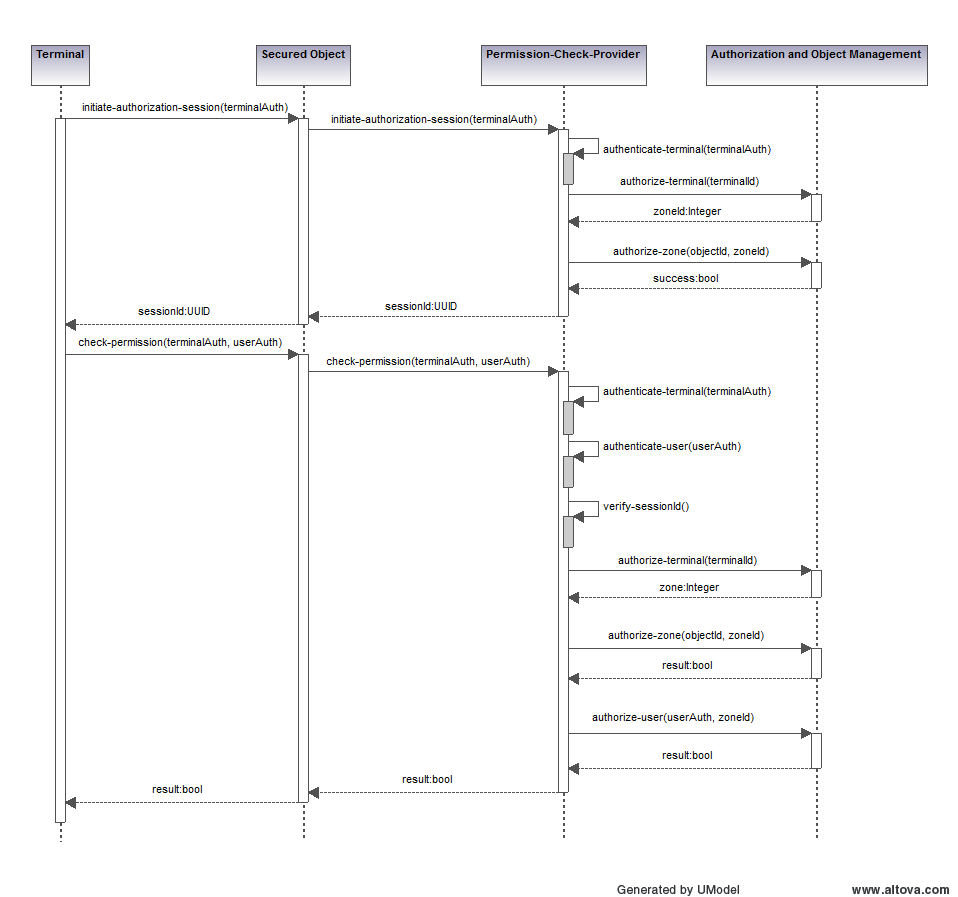
\includegraphics[width=15cm]{./imgs/sequence1.png}}
\end{figure}

Overall availability will also be supported by an active supervisory system to detect failures, emergency backup plans to reduce downtime
and regular health-checks conducted on all internal components to prevent failure at all, at least in certain cases.


\section{lab1b - Interface Definitions}

Tarpit sodass man nicht Brute-forcen kann

Authorization and Object Management hat die Zertifikate der Secured Objects und eventuell auch Terminals (zur Authentifizierung)

Was muss dem Gesetz nach gelogged werden?





\section{lab1c - Security Analysis}


%%%%%%%%%%%%%%%%%%%%%%%%%%%%%%%%%%%%%%%%%%%%%%%%%%%%%%%%%%%%%%%%%%%%%%
%
% DO NOT CHANGE THE FOLLOWING PART
%
%%%%%%%%%%%%%%%%%%%%%%%%%%%%%%%%%%%%%%%%%%%%%%%%%%%%%%%%%%%%%%%%%%%%%%

\end{document}


